This section describes how to install/setup the Netinf NRS and the NetInf Streaming on a server, it is intended for both end users and developers.


\subsection{Dependencies}

In order to run the system properly the following components are required to be installed on the system, the user can either run the script from the section below, or install these manually. Furthermore, the developers support Ubuntu 12.04 LTS 32 bit. Attempts to run this software on other operating systems and architectures may produce unexpected results.


For the NetInf NRS system:
\begin{itemize}
\item Make
\item Rebar
\item G++ compiler
\item Erlang - version R15B03
\end{itemize}

For the NetInf Video Streaming, in addition to the above the following component(s) are required
\begin{itemize}
\item Google Chrome Web browser - or any other browser that supports HTML 5 video tag.
\end{itemize}

To install Make and G++ manually please run the following commands in the terminal.
\begin{verbatim}
sudo apt-get install build-essential
sudo apt-get install g++
\end{verbatim}

To install Rebar and Erlang manually please follow the following steps

Download and install: Rebar from Github
https://github.com/basho/rebar/archive/master.zip

unzip the archive and run the following command
\begin{verbatim}
 cd rebar-master
 ./bootstrap
 sudo cp rebar /usr/bin
 
\end{verbatim}

To Download and install Erlang - version R15B03 for the 32 bit architecture.
It can be retrieved from the Erlang-Solutions website or use the following commands.

\begin{verbatim}

wget https://elearning.erlang-solutions.com/couchdb//rbingen_adapter//package_R15B03_precise32_1354121173/esl-erlang_15.b.3-1~ubuntu~precise_i386.deb
 
sudo dpkg -i esl-erlang_15.b.3-1~ubuntu~precise_i386.deb

\end{verbatim}

\subsection{Script}
\label{backend-install-script}
For the convenience of end users and developers, there is a packaged install/setup script available after obtaining the backend code. This script is responsible for quickly installing the entire system with all the dependencies.

\textbf{If the script is not immediately runnable please run the following command:}
\begin{verbatim}
chmod a+x netinf_nrs.sh
\end{verbatim}

The script can be run by using the following on a command line terminal.

\begin{verbatim}
./netinf_nrs.sh
\end{verbatim}

The script will be put a into a menu loop shown below and instructs the user to type a number in order to choose an option.Choosing an option will preform the task and then cause the script to exit normally.

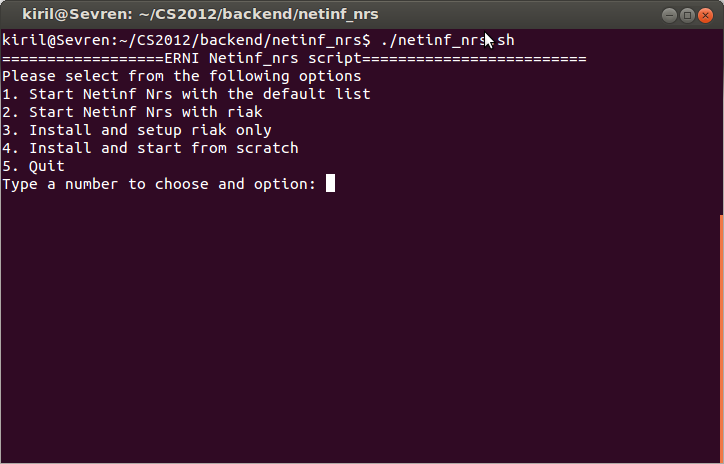
\includegraphics[scale=0.5]{./img/Backend_install_script.png}

The following options are available to the user

\begin{itemize}
\item Start Netinf NRS with the default list\\
Assumes the system has all the dependencies installed and only starts the NetInf NRS with the list database.
\item Start Netinf NRS with riak\\
Will check that Riak is running and present in the system and then start the NetInf NRS with the Riak database.
If riak is not present then the script will download and install all the required components. 
\item Install and setup riak only\\
Use this option only when Riak needs to be downloaded and installed on the machine. This will not start an NRS.
\item Install and start from scratch\\
This option assumes a bare machine and checks that all the dependencies are satisfied. It will auto download and install anything that is required and then start the NetInf NRS with the default list database. 
\end{itemize}


\subsection{Riak Database}

Riak is a database written in Erlang. It is known for being distributed and fault-tolerant. Riak was chosen above other database implementations since it was suggested by the client and the development team had great support available. 

In case there is something wrong with the script process on the target machine please follow the manual installation instructions below.

Install libssl0.9.8 with:
\begin {verbatim}
sudo apt-get install libssl0.9.8
\end{verbatim}

Next install the Riak database:
\begin{verbatim}
wget http://downloads.basho.com.s3-website-us-east-1.amazonaws.com/riak/CURRENT/ubuntu/lucid/riak_1.2.1-1_i386.deb
sudo dpkg -i riak_1.2.1-1_i386.deb
\end{verbatim}

In order for the search to work in the Riak system and from the NRS please enable search.
Riak Search is enabled in the app.config (/etc/riak/app.config) file. Simply change the setting to “true” in Riak Search Config section (shown below).

\begin{verbatim}
%% Riak Search Config
{riak_search, [
               %% To enable Search functionality set this 'true'.
               {enabled, false}
              ]},
\end{verbatim}

Then run the in the terminal;

\begin{verbatim}
riak restart
\end{verbatim}

Followed by the command below to index the bucket:

\begin{verbatim}
search-cmd install netinf_bucket
\end{verbatim}

Lastly, please make sure that the NRS is started with the Riak database.

\subsection{Running the NetInf NRS}

To run the NetInf NRS without the script, please run the following commands after navigating to the netinf\_nrs folder:

\begin{itemize}
\item Using the list database \\
\begin{verbatim}
erl -pa ebin deps/*/ebin -config configs/list -s netinf_nrs 
-eval "io:format(\"NetInf NRS is running ... ~n\")." 
\end{verbatim}

\item Using the riak databse \\
Please make sure the Riak daemon is started before. If it has not been started use the first command shown below before the erl command.
\begin{verbatim}
riak start

erl -pa ebin deps/*/ebin -config configs/riak -s netinf_nrs 
-eval "io:format(\"NetInf NRS is running ... ~n\")." 
\end{verbatim}
\end{itemize}